
\section{Empirical Results}

\begin{frame}{Example 1 - Standard and Poor's (S\&P) 500 index}

    Daily S\&P 500 index from Federal Reserve Economic Data (\cite{SP500})

    \begin{itemize}
    \item February 11, 2013 - February 10, 2023
    \item $T = 2519$
    \item $R = 1511$ (60\%)
    \item $P = 1008$
    \end{itemize}

    \vspace{4mm}
    
    We focus on three common classes of linear time series models: 
    
    \begin{itemize}
    \item Autoregressive integrated moving average (ARIMA)
    \item Exponential smoothing (ETS)
    \item Linear regression model with ARIMA errors
    \end{itemize}

\end{frame}



\begin{frame}[plain]{}
\begin{figure}[ht]
\centering
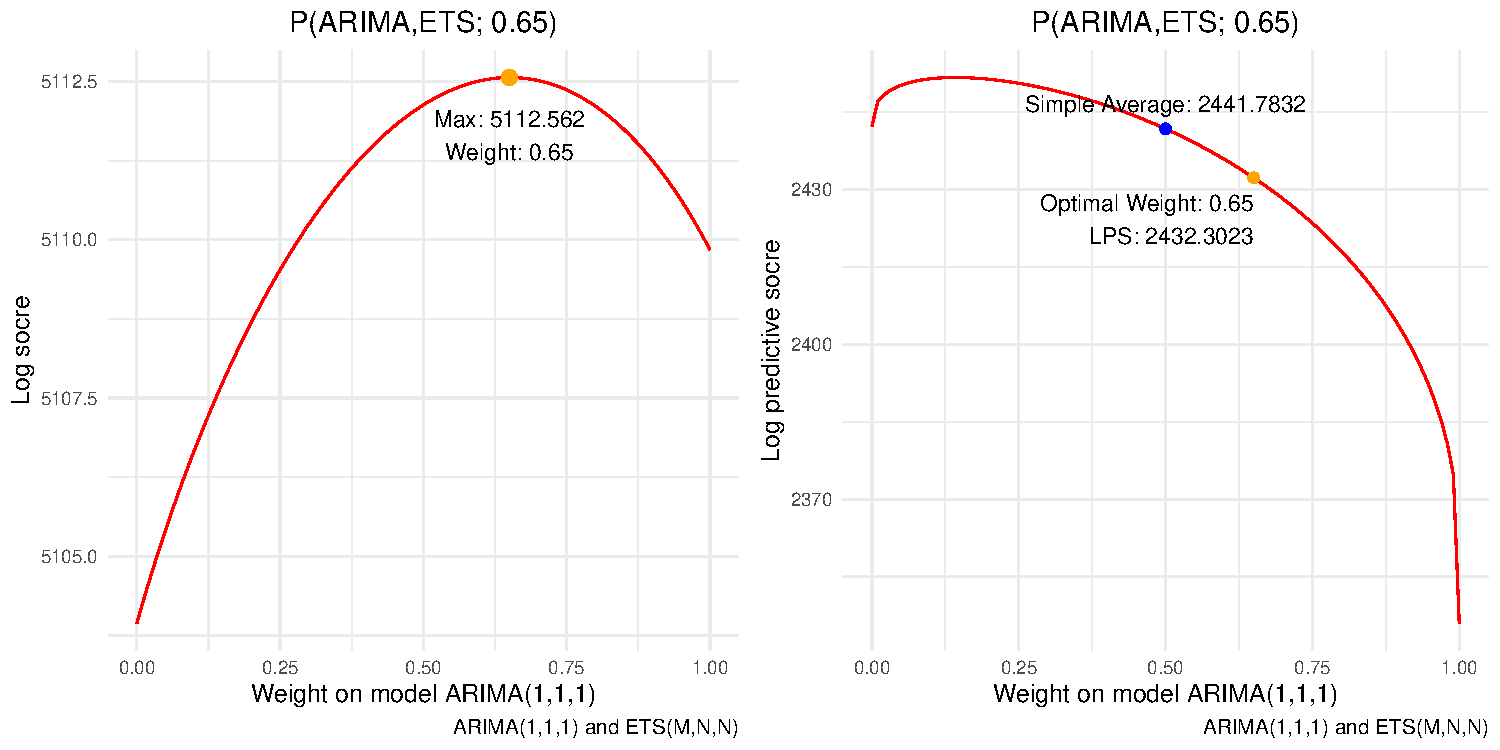
\includegraphics[scale=0.55]{Graph/SP500_nonstat_1.pdf}
\caption{\footnotesize{Log score of S\&P 500 index predictive densities in P(ARIMA, ETS; 0.65).}}
\end{figure}
\end{frame}



\begin{frame}[plain]{}
\begin{figure}[ht]
\centering
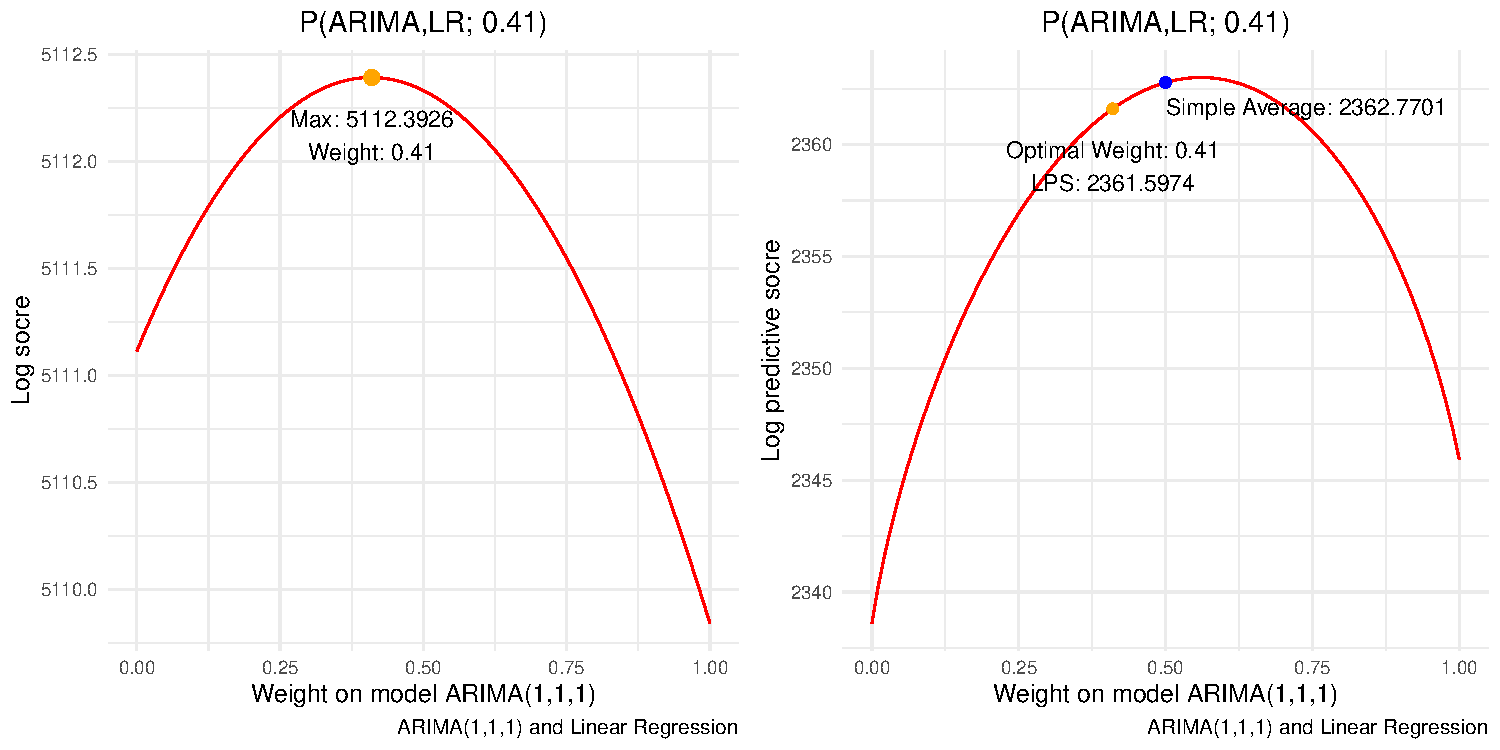
\includegraphics[scale=0.55]{Graph/SP500_nonstat_2.pdf}
\caption{\footnotesize{Log score of S\&P 500 index predictive densities in P(ARIMA, LR; 0.41).}}
\end{figure}
\end{frame}



\begin{frame}[plain]{}
\begin{figure}[ht]
\centering
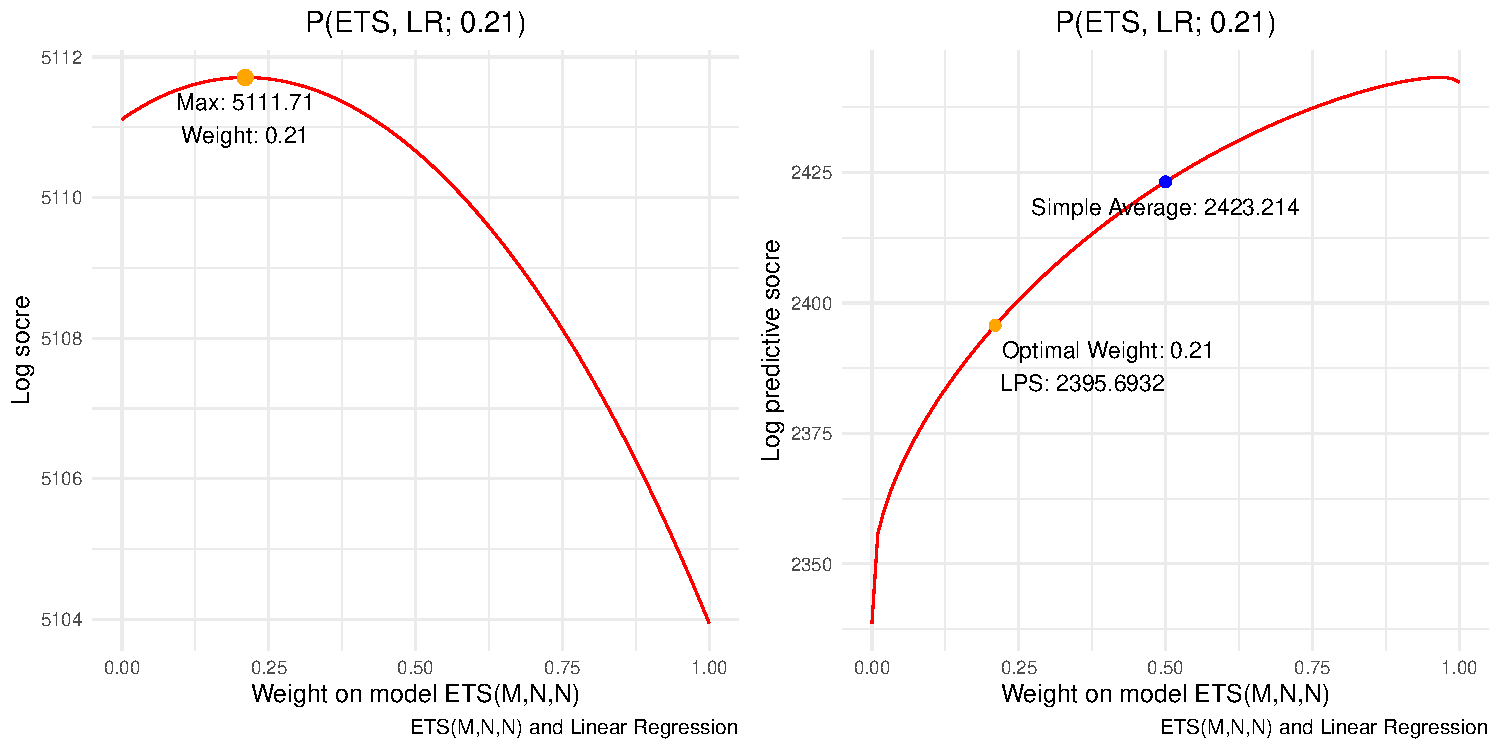
\includegraphics[scale=0.55]{Graph/SP500_nonstat_3.pdf}
\caption{\footnotesize{Log score of S\&P 500 index predictive densities in P(ETS, LR; 0.21).}}
\end{figure}
\end{frame}



\begin{frame}{In-sample Fit Comparison}

\begin{table}[ht]
  \centering
    \begin{tabular}{l<{\onslide<1->}|c>{\onslide<2->}c>{\onslide<3->}c<{\onslide<1->}}
    \toprule
    &    P(ARIMA,ETS; 0.65)     &   P(ARIMA,LR; 0.41)    &    P(ETS,LR; 0.21)   \\  
    \midrule
    $1^{st}$ Model LogL    &     5113.694       &    5113.694    &   1725.137     \\
    $2^{nd}$ Model LogL    &     1725.137       &    5116.014    &   5116.014     \\
    Difference             &     3388.556       &     2.320      &   3390.876     \\
    Puzzle                 &       Yes          &      Yes       &     Yes        \\
    \bottomrule
    \end{tabular}
\end{table}

\begin{columns}[t]
    \begin{column}{0.6\textwidth}
        \begin{table}
            \centering
            \scalebox{0.9}{
            \begin{tabular}{l<{\onslide<1->}|c>{\onslide<2->}c>{\onslide<3->}c<{\onslide<1->}}
            \toprule
            &    P(ARIMA,ETS)     &   P(ARIMA,LR)    &    P(ETS,LR)   \\  
            \midrule
            Type    &   (G,B)   &  (G,G)   & (B,G)   \\
            Puzzle  &   Yes     &   Yes    &  Yes    \\
            \bottomrule
            \end{tabular}}
        \end{table}
    \end{column}
    
    \begin{column}{0.4\textwidth}
        \begin{table}
            \centering
            \scalebox{0.9}{
            \begin{tabular}{cccc}
                                   &      & \multicolumn{2}{c}{$M_2$} \\
                                   &      & Good       & Bad       \\
            \multirow{2}{*}{$M_1$} & Good & \alt<2>{\alert{$\surd$}}{$\surd$}    & \alt<1>{\alert{$?$}}{$?$} \\
                                   & Bad  & \alt<3>{\alert{$?$}}{$?$}       & $\surd$
            \end{tabular}}
        \end{table}
    \end{column}
    \end{columns}
    
\end{frame}



\begin{frame}{Example 1 - S\&P 500 log returns}

Same dataset but modelling the S\&P 500 log returns

\begin{table}[ht]
  \centering
    \begin{tabular}{l|ccc}
    \toprule
                                      &        P(ARMA,LR;0.69)    \\  
    \midrule
    $1^{st}$ model Log Likelihood     &         5109.8071         \\
    $2^{nd}$ model Log Likelihood     &         5109.8054         \\
    Puzzle                            &           Yes             \\
    \bottomrule
    \end{tabular}
\end{table}
\end{frame}



\begin{frame}[plain]{}
\begin{figure}[ht]
\centering
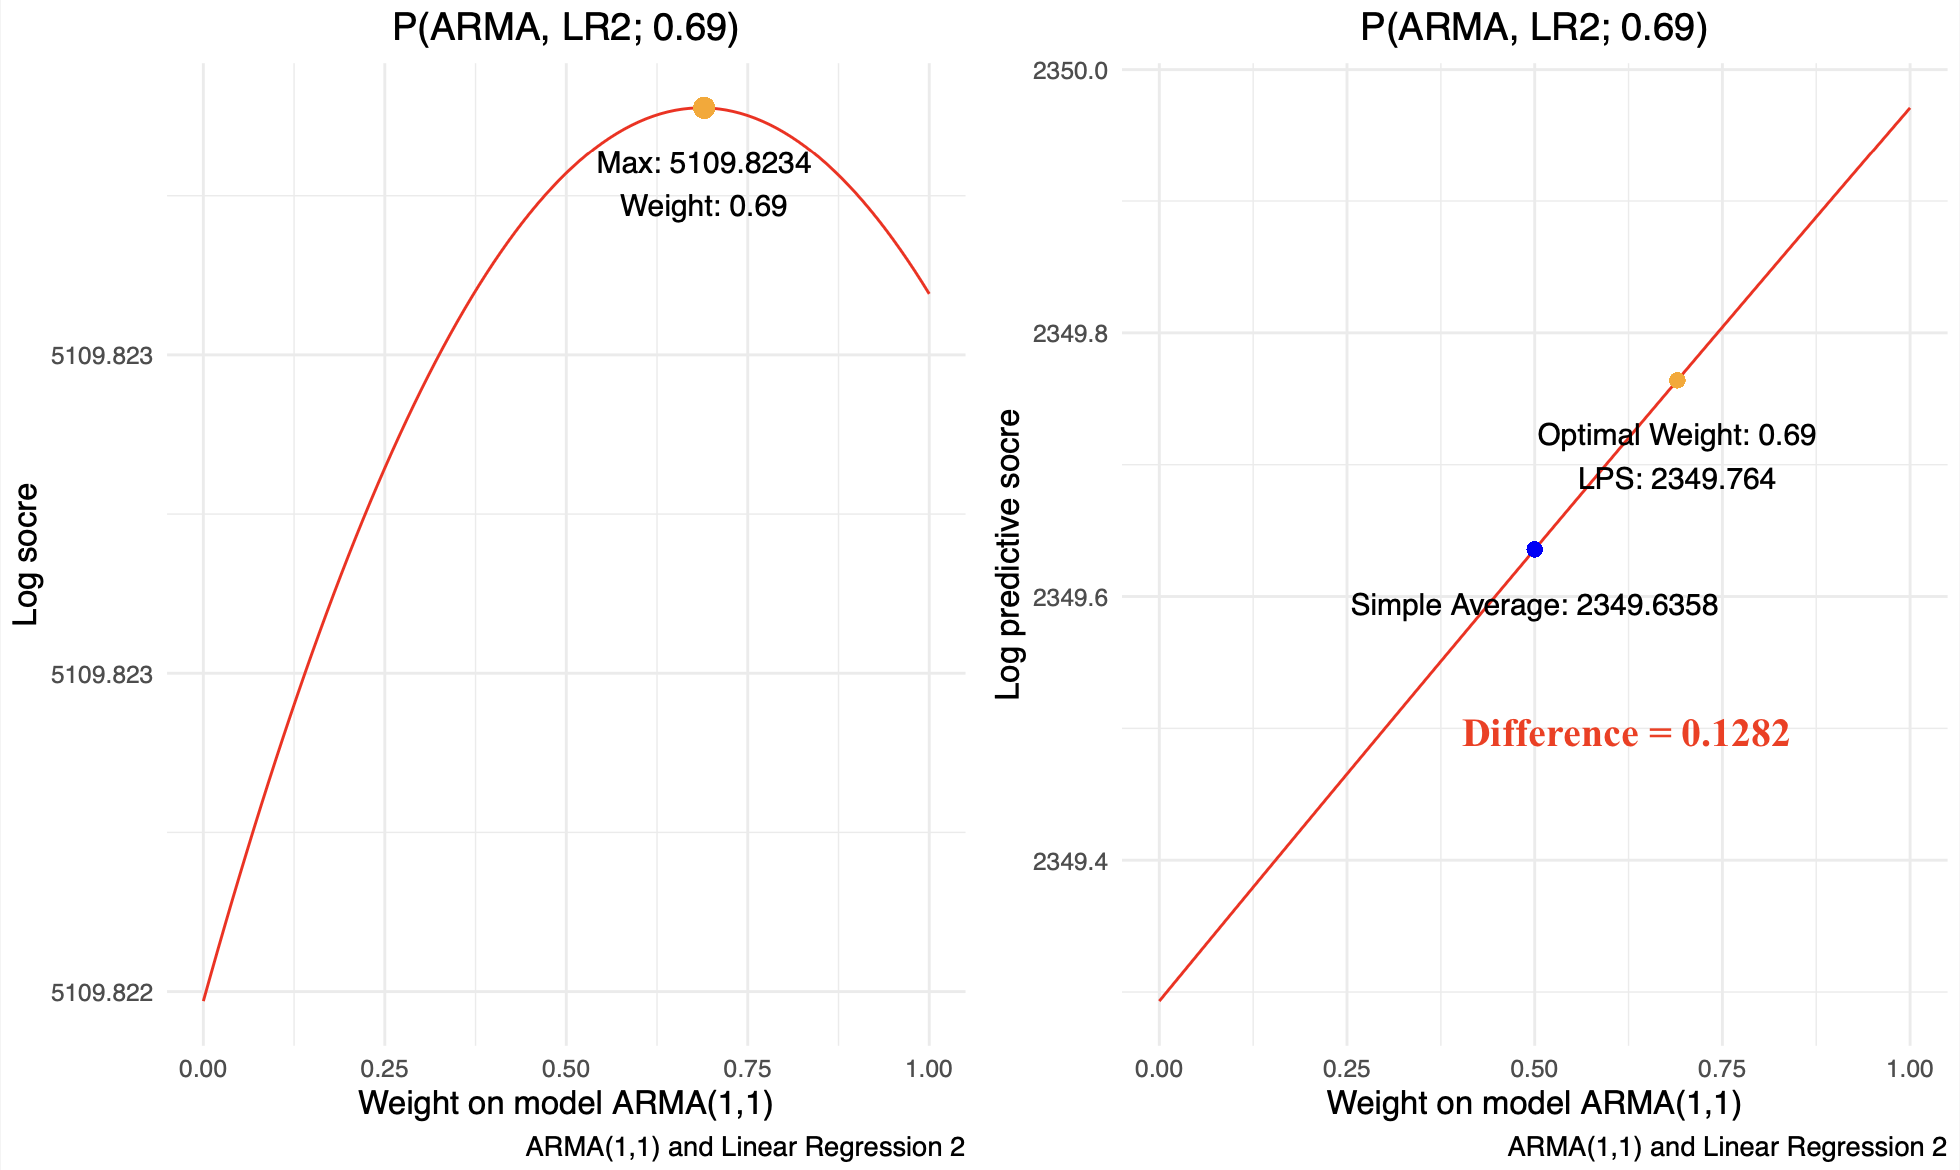
\includegraphics[scale=0.37]{Graph/SP500_stationary.png}
\caption{\footnotesize Log score of S\&P 500 log returns predictive densities in two-model pools.}
\end{figure}
\end{frame}



\begin{frame}{Example 2 - Seasonal Number of Unemployment}
    Quarterly total number of unemployed individuals (in thousands) retrieved from the Australia Bureau of Statistics (\cite{ABS})

    \begin{itemize}
    \item 1985 Q1 - 2023 Q1
    \item $T = 2519$
    \item $R = 1511$ (60\%)
    \item $P = 1008$
    \end{itemize}

    \vspace{5mm}
    
    We now consider the following linear time series models: 
    
    \begin{itemize}
    \item Seasonal autoregressive integrated moving average (SARIMA)
    \item Exponential smoothing (ETS)
    \end{itemize}
\end{frame}



\begin{frame}[plain]{}

\begin{columns}
    \begin{column}{0.5\textwidth}
        \begin{figure}[ht]
        \centering
        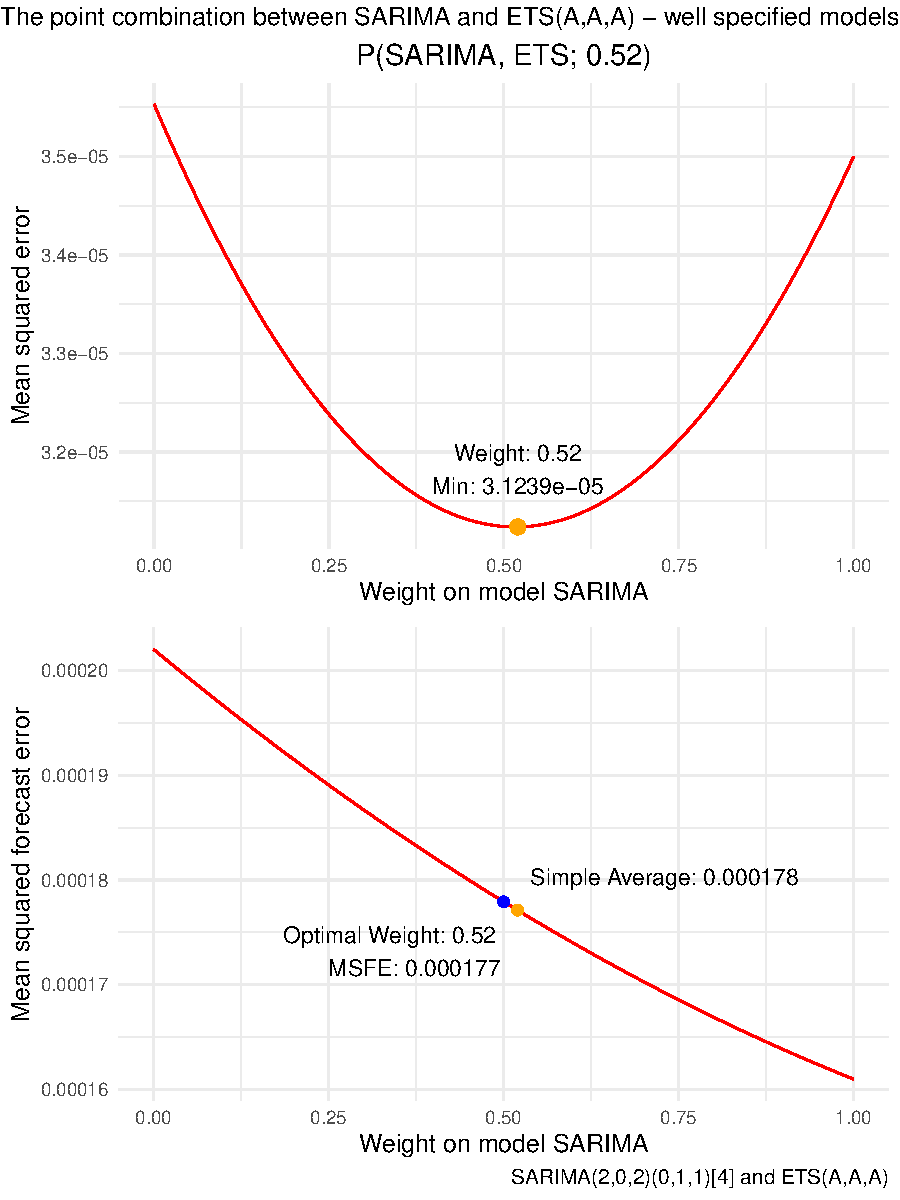
\includegraphics[scale=0.37]{Graph/EMPL_correct.pdf}
        \caption{\footnotesize{MSFE of predictive unemployment in two well-specified model pools.}}
        \end{figure}
    \end{column}
    
    \begin{column}{0.5\textwidth}
        \begin{figure}[ht]
        \centering
        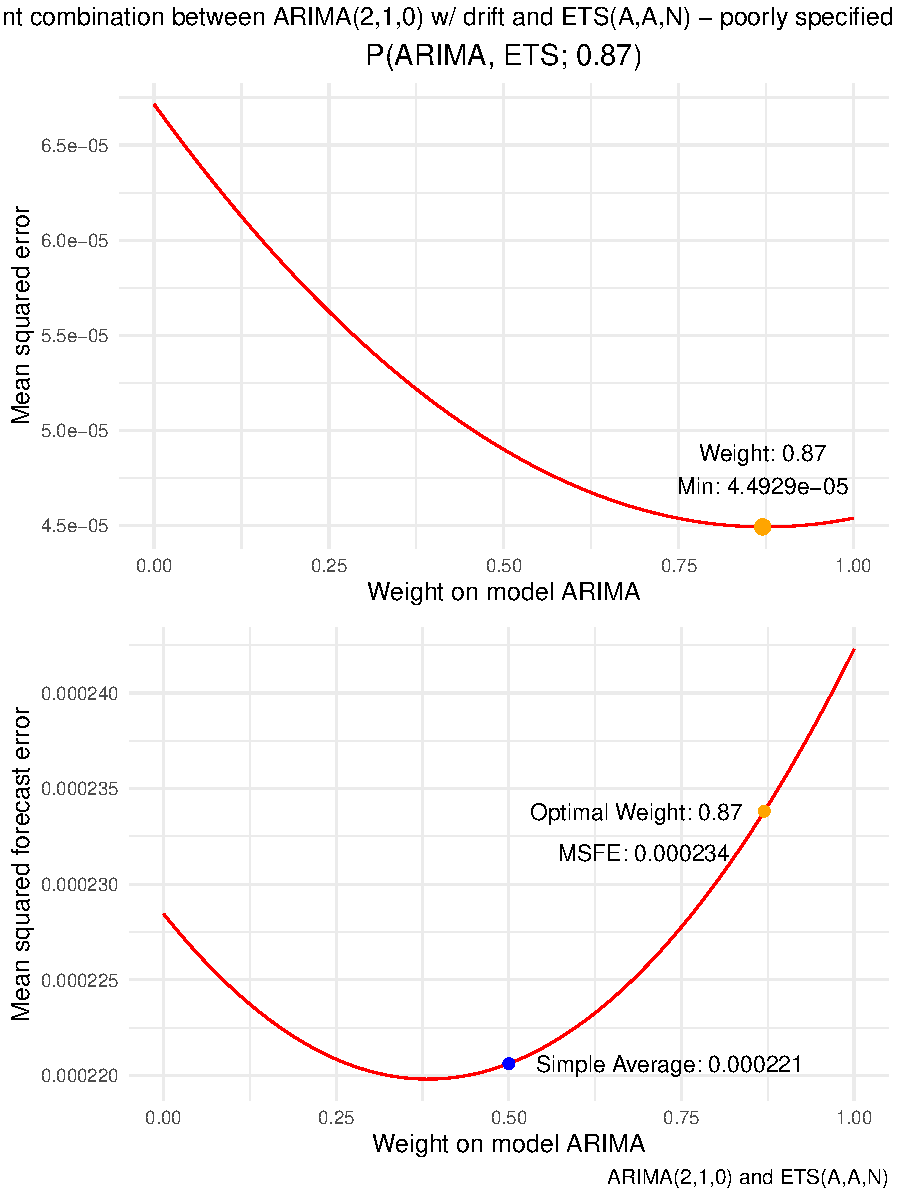
\includegraphics[scale=0.37]{Graph/EMPL_misspecified.pdf}
        \caption{\footnotesize{MSFE of predictive unemployment in two poorly-specified model pools.}}
        \end{figure}
    \end{column}
    \end{columns}

\end{frame}



\begin{frame}{Example 2 - In-sample Fit Comparison}

\begin{table}[ht]
  \centering
    \begin{tabular}{l|ccc}
    \toprule
        &   P(SARIMA,ETS;0.52)   &   P(ARIMA,ETS;0.87)  \\  
    \midrule
    $1^{st}$ Model LogL   &   321.4497   &    322.1642   \\
    $2^{nd}$ Model LogL   &   260.9102   &    231.9507   \\
    Difference            &   60.5395    &    90.2135    \\
    Puzzle                &    Yes       &     Yes       \\
    \bottomrule
    \end{tabular}
\end{table}
\end{frame}



\begin{frame}{Conjecture Revision}

    Under a mild definition of the forecast combination puzzle, the empirical evidence suggest that the puzzle is in evidence in all the cases.
    
    \begin{table}
    \centering
    \begin{tabular}{cccc}
           &      & \multicolumn{2}{c}{$M_2$} \\
           &      & Good       & Bad       \\
    \multirow{2}{*}{$M_1$} & Good & $\surd$  & $\surd$ \\
                           & Bad  & $\surd$  & $\surd$
    \end{tabular}
    \end{table}

    However, there are too few examples to draw conclusions.

    We may encounter situations where the optimal forecast combination is more accurate than the simple averaging.

\end{frame}

